\subsection{Numerical results}
\label{subsec:numerical-second-order}
We apply the second-order discretization to the same manufactured
solution, forcing, parameters, and meshes specified in
\Cref{subsec:revised-numerical-first}, retaining $T=2$ and $\dt=1/K$.
Velocity and angular velocity now use continuous piecewise quadratic
elements, pressure remains continuous piecewise linear, magnetization
uses RT1, and $\bs z,\bs k,\bs H$ use first-family Nedelec elements
one degree above the lowest order. The scalar fields
$\varphi,\vartheta,\varpi$ are continuous piecewise quadratic.
The corresponding RT and Nedelec Basix degree is two.

The first time step is solved by a Broyden quasi-Newton iteration with
relative tolerance $10^{-9}$ and a maximum of 12 iterations.
The accepted state is checked by reassembling the nonlinear midpoint
equations. Subsequent time steps use the prescribed extrapolated
coefficients and require one five-block linear solve per step.
The $\bs z_h$ and $\varpi_h$ slots represent the current midpoint-stage
projections; they are not averaged again with the preceding stage.

The primary fields are compared at $T$. The pressure slot represents
the averaged modified pressure, so its reference is
\[
\widetilde p_{\mathrm{ref}}^{N-1/2}
=\frac{\widetilde p(T)+\widetilde p(T-\dt)}{2},
\]
with the same zero-mean convention as above. This reference is not
identified with either the endpoint pressure or the analytic pressure
evaluated directly at the midpoint.

\Cref{tab:second-order-errors,fig:second-order-convergence} show that
the finest-grid rates for $\bs u,\widetilde p,\bs\omega,\bs m,
\varphi,\bs H$ are 2.166, 2.051, 1.981, 2.007, 1.968, and 1.968,
respectively. The $L^2$ error of $\bs k$ decreases approximately at
first order, with a finest-grid rate of 1.015; second-order convergence
is therefore not claimed for every auxiliary quantity.
The sampled curl diagnostic ranges from $7.30\times10^{-13}$ to
$6.96\times10^{-11}$. For $K=32$, all 64 steps reach $T=2$, and
the final full-system relative algebraic residual is
$2.08\times10^{-13}$.
These observations support the reported joint-refinement behavior.
Because the mesh and time step vary together and the primary exact
fields have linear temporal amplitudes, they do not constitute a
separate test of pure temporal accuracy or of energy stability.

\begin{table}[htbp]
\centering
\caption{Relative errors and observed rates for the second-order scheme, $T=2$ and $\dt=1/K$. $C_H$ is the sampled absolute curl diagnostic.}
\label{tab:second-order-errors}
\begingroup
\small
\setlength{\tabcolsep}{3.5pt}
\renewcommand{\arraystretch}{1.15}
\begin{tabular}{crrrrrrrr}
\toprule
\multicolumn{9}{c}{(a) Velocity, pressure, angular velocity, and magnetization}\\
\midrule
$K$ & \multicolumn{2}{c}{$\bs u$: $H^1$} & \multicolumn{2}{c}{$\widetilde p$: $L^2$} & \multicolumn{2}{c}{$\bs\omega$: $H^1$} & \multicolumn{2}{c}{$\bs m$: $H(\div)$}\\
 & Error & Rate & Error & Rate & Error & Rate & Error & Rate\\
\midrule
4 & $5.6873\!\times\!10^{-1}$ & -- & $4.2000\!\times\!10^{-1}$ & -- & $2.1381\!\times\!10^{-1}$ & -- & $1.1937\!\times\!10^{-1}$ & --\\
8 & $1.5090\!\times\!10^{-1}$ & 1.914 & $9.4815\!\times\!10^{-2}$ & 2.147 & $6.2017\!\times\!10^{-2}$ & 1.786 & $3.1613\!\times\!10^{-2}$ & 1.917\\
16 & $2.4805\!\times\!10^{-2}$ & 2.605 & $2.0872\!\times\!10^{-2}$ & 2.184 & $1.6320\!\times\!10^{-2}$ & 1.926 & $7.8383\!\times\!10^{-3}$ & 2.012\\
32 & $5.5259\!\times\!10^{-3}$ & 2.166 & $5.0382\!\times\!10^{-3}$ & 2.051 & $4.1345\!\times\!10^{-3}$ & 1.981 & $1.9494\!\times\!10^{-3}$ & 2.007\\
\bottomrule
\end{tabular}
\par\medskip
\begin{tabular}{crrrrrrr}
\toprule
\multicolumn{8}{c}{(b) Auxiliary curl field, potential, magnetic field, and curl diagnostic}\\
\midrule
$K$ & \multicolumn{2}{c}{$\bs k$: $L^2$} & \multicolumn{2}{c}{$\varphi$: $H^1$} & \multicolumn{2}{c}{$\bs H$: $H(\curl)$} & $C_H$\\
 & Error & Rate & Error & Rate & Error & Rate &\\
\midrule
4 & $2.1008\!\times\!10^{-1}$ & -- & $2.0119\!\times\!10^{-1}$ & -- & $2.0303\!\times\!10^{-1}$ & -- & $7.3001\!\times\!10^{-13}$\\
8 & $9.5804\!\times\!10^{-2}$ & 1.133 & $6.0098\!\times\!10^{-2}$ & 1.743 & $6.0718\!\times\!10^{-2}$ & 1.742 & $3.9064\!\times\!10^{-12}$\\
16 & $4.6084\!\times\!10^{-2}$ & 1.056 & $1.6119\!\times\!10^{-2}$ & 1.899 & $1.6289\!\times\!10^{-2}$ & 1.898 & $1.8492\!\times\!10^{-11}$\\
32 & $2.2804\!\times\!10^{-2}$ & 1.015 & $4.1189\!\times\!10^{-3}$ & 1.968 & $4.1627\!\times\!10^{-3}$ & 1.968 & $6.9611\!\times\!10^{-11}$\\
\bottomrule
\end{tabular}
\endgroup
\end{table}

\begin{figure}[htbp]
\centering
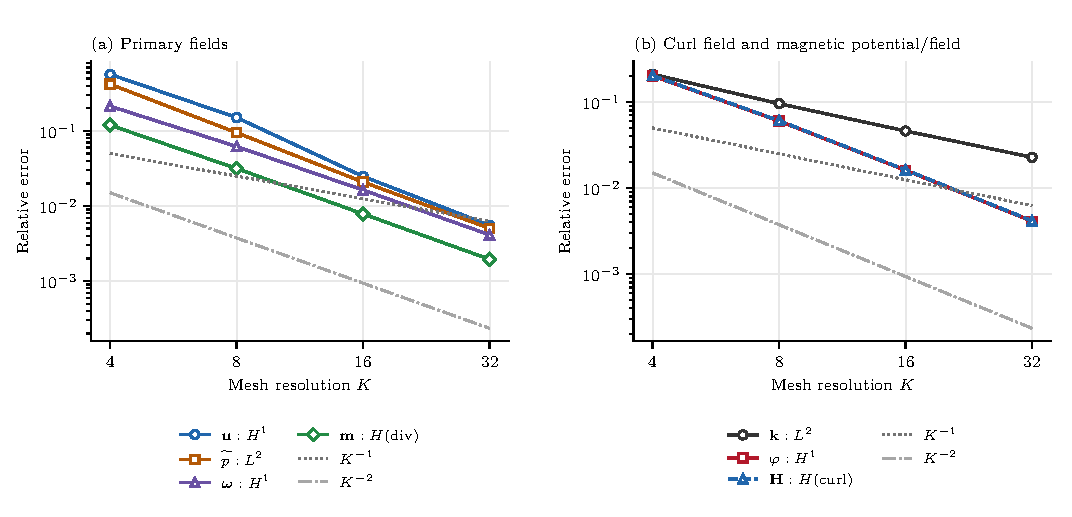
\includegraphics[width=\textwidth]{figures/second_order_errors.pdf}
\caption{Relative errors for the second-order discretization using the
same manufactured solution and $\dt=1/K$.
(a) Velocity, averaged modified pressure, angular velocity, and magnetization.
(b) Auxiliary curl field, magnetic potential, and magnetic field.
The horizontal coordinate is $K=4,8,16,32$, increasing from left to
right. Reference lines proportional to $K^{-1}$ and $K^{-2}$ distinguish
the nearly quadratic decay of the principal errors from the
approximately first-order $L^2$ decay for $\bs k$.}
\label{fig:second-order-convergence}
\end{figure}

\subsubsection{Second-order scheme}
\label{subsec:second-order-energy}
\Cref{fig:second-order-energy} shows monotone energy decay for all
three time steps, with initial energy approximately
$4.295033\times10^{-2}$.
\Cref{tab:second-order-energy} reports the final ratios and balance
diagnostics; the largest normalized balance defect is
$3.71\times10^{-11}$.
The coarsest time step produces slower late-time decay, which is
retained in the plot. Energy dissipation therefore should not be
interpreted as evidence that the temporal error is negligible.
Since the two schemes also use different spatial approximation
orders, these figures are separate stability tests rather than
a controlled comparison of temporal accuracy. The computations
provide numerical evidence of the discrete dissipation mechanism
at the tested step sizes, not a proof for arbitrary step sizes.

\begin{table}[htbp]
\centering
\caption{Second-order unforced energy test: $K=8$, $T=0.5$.}
\label{tab:second-order-energy}
\small
\begin{tabular}{crr}
\toprule
$\dt$ & $E_h(T)/E_h(0)$ & $\max_n\epsilon_{\rm bal}^n$\\
\midrule
$1/16$ & $1.1117\times10^{-4}$ & $3.71\times10^{-11}$\\
$1/32$ & $2.5984\times10^{-5}$ & $7.77\times10^{-13}$\\
$1/64$ & $1.0438\times10^{-5}$ & $2.67\times10^{-13}$\\
\bottomrule
\end{tabular}
\end{table}

\begin{figure}[htbp]
\centering
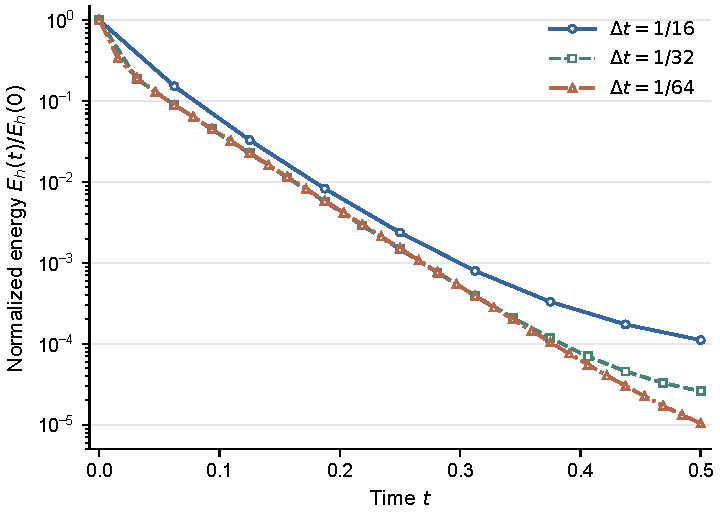
\includegraphics[width=0.70\textwidth]{figures/second_order_energy.pdf}
\caption{Normalized discrete energy for the second-order scheme in the
unforced relaxation test, $K=8$ and $T=0.5$.
The logarithmic vertical scale matches \Cref{fig:first-order-energy}.
Symbols represent all computed time levels without smoothing.
The same discrete initial state is used for all three time steps.}
\label{fig:second-order-energy}
\end{figure}
\FloatBarrier

